\documentclass[tikz]{standalone}

\usepackage[english,russian]{babel}
\usepackage[T2A,T1]{fontenc}
\usepackage[utf8]{inputenc}
\tikzset{
	force/.style=	{
		>=latex,
		draw=blue,
		fill=blue,
				 	}, 
	%				 	
	axis/.style=	{
		densely dashed,
		blue,
		line width=1pt,
		font=\small,
					},
	%
	th/.style=	{
		line width=1pt},
	%
	acceleration/.style={
		>=open triangle 60,
		draw=magenta,
		fill=magenta,
					},
	%
	inforce/.style=	{
		force,
		double equal sign distance=2pt,
					},
	%
	interface/.style={
		pattern = north east lines, 
		draw    = none, 
		pattern color=gray!60,
					},
	cross/.style=	{
		cross out, 
		draw=black, 
		minimum size=2*(#1-\pgflinewidth), 
		inner sep=0pt, outer sep=0pt,
					},
	%
	cargo/.style=	{
		rectangle, 
		fill=black!70, 
		inner sep=2.5mm,
					},
	%
	caption/.style= {
		midway,
		fill=white!20, 
		opacity=0.9
					},
	%
	}
\usepackage
    {
        tikz,
        pgfplots,
        verbatim,
    }
\usetikzlibrary
    {
        arrows,
        patterns,
        angles,
        quotes,
        calc, 
        3d,  
        backgrounds, 
        positioning
    }
\usetikzlibrary{fadings,through}
\tikzset
    {
        media/.style={font={\footnotesize\sffamily}},
        wave/.style={
            decorate,decoration={snake,post length=1.4mm,amplitude=2mm,
                segment length=1mm},thick},   
    }
\begin{document}
\begin{tikzpicture}[scale=1.5]
	% \xdef\darkness{0}
	% \xdef\op{0.1}

	% \xdef\SIZE{5}

    \node[inner sep=0pt] (russell) at (0,0)
        {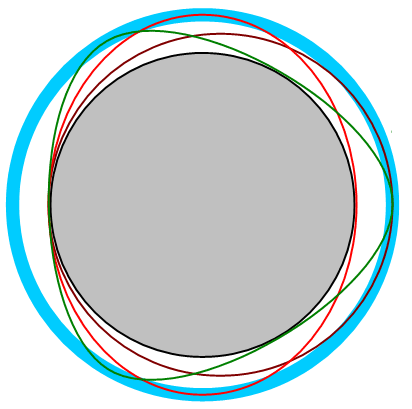
\includegraphics[width=.25\textwidth]{sh.png}};
	% \draw[step=1.0,blue,thick,opacity=\op] (0,0) grid (\SIZE,\SIZE);
	% \draw[step=0.5,blue,very thin,opacity=\op] (0,0) grid (\SIZE,\SIZE);

	% \foreach \i in {0,1,...,\SIZE} {
 %    	\draw[opacity=\op] (0,\i) node [left] {\i};
 %    	\draw[opacity=\op] (\i,0) node [below] {\i};
 %    }

    % \draw[xshift=2cm, fill=black!10] (0,0) arc (0:180:2) -- cycle; 

    % % \draw[xshift=4cm, dashed, opacity=0.7] (0,0) arc (0:180:4); 

    % \foreach \i in {0,5,...,180} {
    %     \draw[] (\i:3.5) node [align=center] {+};
    % }


    \node [align=center] () at (0,0) {Земля};
    \node [align=center] () at (0,1.1) {Ионосфера};
    % \node [align=center, above, yshift=1em] () at (0,3.5) {Ионосфера};

    % \foreach \i in {0,10,...,180} {
    %     \draw[] (\i:1.8) node [align=center] {-};
    % }

    % \draw[->] (60:2.2) -- node[right, align=center, opacity=1] {Ток \\ молний}  (60:3.3) ;
    % \draw[->] (120:2.2) -- node[left, align=center, opacity=1] {Ток \\ осадков}  (120:3.3) ;
    % \draw[<-] (90:2.2) -- node[right, align=center, opacity=1] {Ток \\хорошей\\ погоды}  (90:3.3) ;

% \begin{scope}[xshift=3cm]
%     \draw [thick] (0,0) node [left] {$E_1$} -- ++(2,0);
%     \draw [thick] (0,2.5) node [left] {$E_2$} -- ++(2,0);
%     % \draw[thick,->] (1,2.5) -- (1,5pt);
%     % \draw[dashed, fill=white] (1,2.5) circle (5pt);

%     \draw[fill=black] (1,0) circle (5pt);
% 	\draw [decorate, magenta, decoration={snake}, ->] (1,1.25) --
%     node [below,sloped]{$h\nu$} ++(1,0); 
% \end{scope}

	% \node [align=center] () at (-3+1,-1) {Возбужденное \\ состояние атома};
	% \node [align=center] () at (3+1,-1) {Основное \\ состояние атома};

	% \node [align=center] () at (-3+1,2.5+1) {До эмиссии};
	% \node [align=center] () at (0+1,2.5+1) {Эмиссия};
	% \node [align=center] () at (3+1,2.5+1) {После эмиссии};


\end{tikzpicture} 
\end{document}
